% This file was created with tikzplotlib v0.10.1.
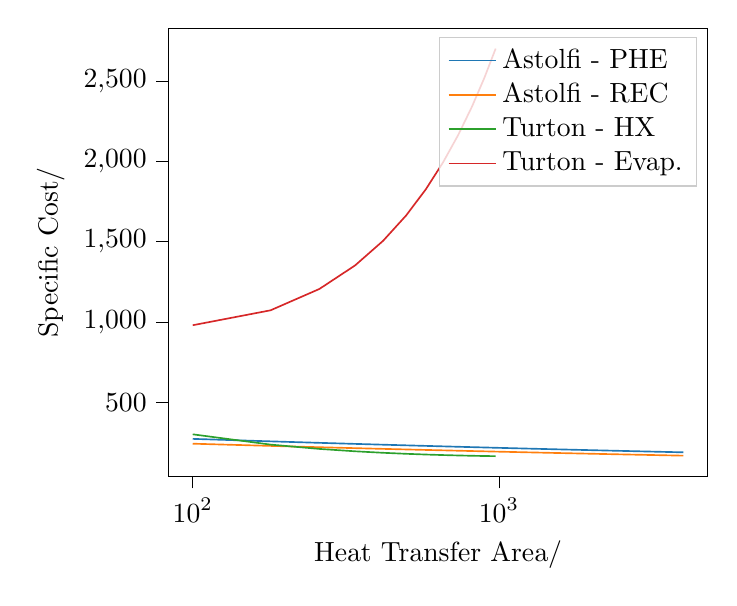
\begin{tikzpicture}

\definecolor{crimson2143940}{RGB}{214,39,40}
\definecolor{darkgray176}{RGB}{176,176,176}
\definecolor{darkorange25512714}{RGB}{255,127,14}
\definecolor{forestgreen4416044}{RGB}{44,160,44}
\definecolor{lightgray204}{RGB}{204,204,204}
\definecolor{steelblue31119180}{RGB}{31,119,180}

\begin{axis}[
legend cell align={left},
legend style={fill opacity=0.8, draw opacity=1, text opacity=1, draw=lightgray204},
log basis x={10},
tick align=outside,
tick pos=left,
unbounded coords=jump,
x grid style={darkgray176},
xlabel={Heat Transfer Area/\unit{\square\m}},
xmin=83.1566529016914, xmax=4810.19841518734,
xmode=log,
xtick style={color=black},
xtick={1,10,100,1000,10000,100000},
xticklabels={
  \(\displaystyle {10^{0}}\),
  \(\displaystyle {10^{1}}\),
  \(\displaystyle {10^{2}}\),
  \(\displaystyle {10^{3}}\),
  \(\displaystyle {10^{4}}\),
  \(\displaystyle {10^{5}}\)
},
y grid style={darkgray176},
ylabel={Specific Cost/\unit{\USD\per\square\m}},
ymin=37.0151704033557, ymax=2830.58725063895,
ytick style={color=black}
]
\addplot [semithick, steelblue31119180]
table {%
100 271.792373879136
179.591836734694 256.335412463815
259.183673469388 247.102137833008
338.775510204082 240.572546921325
418.367346938775 235.549121455437
497.959183673469 231.482355103319
577.551020408163 228.075287670903
657.142857142857 225.149655969404
736.734693877551 222.590258929937
816.326530612245 220.318454152949
895.918367346939 218.278229684151
975.510204081633 216.428318457775
1055.10204081633 214.737464330224
1134.69387755102 213.18144208414
1214.28571428571 211.741106519046
1293.87755102041 210.401072408877
1373.4693877551 209.148795810205
1453.0612244898 207.973918945329
1532.65306122449 206.867793011582
1612.24489795918 205.823124029771
1691.83673469388 204.833705606609
1771.42857142857 203.894214266297
1851.02040816327 203.000050596001
1930.61224489796 202.14721445338
2010.20408163265 201.332205851853
2089.79591836735 200.55194544845
2169.38775510204 199.803710169799
2248.97959183673 199.085080652726
2328.57142857143 198.393897995841
2408.16326530612 197.728227915288
2487.75510204082 197.086330837635
2567.34693877551 196.466636790598
2646.9387755102 195.867724198978
2726.5306122449 195.288301880823
2806.12244897959 194.727193682672
2885.71428571429 194.183325304078
2965.30612244898 193.655712948438
3044.89795918367 193.143453505316
3124.48979591837 192.645716023449
3204.08163265306 192.161734276566
3283.67346938775 191.690800258606
3363.26530612245 191.232258472687
3442.85714285714 190.785500900665
3522.44897959184 190.349962558503
3602.04081632653 189.925117557653
3681.63265306122 189.510475605065
3761.22448979592 189.105578884636
3840.81632653061 188.709999271413
3920.40816326531 188.323335836963
4000 187.945212610227
};
\addlegendentry{Astolfi - PHE}
\addplot [semithick, darkorange25512714]
table {%
100 241.741563692661
179.591836734694 227.993606128044
259.183673469388 219.781211440886
338.775510204082 213.973566823287
418.367346938775 209.505557990348
497.959183673469 205.888434952265
577.551020408163 202.858071013191
657.142857142857 200.255912710458
736.734693877551 197.979496217969
816.326530612245 195.958874258069
895.918367346939 194.144227855994
975.510204081633 192.498852652215
1055.10204081633 190.994948348587
1134.69387755102 189.610968196604
1214.28571428571 188.329883790966
1293.87755102041 187.138010978016
1373.4693877551 186.024192739417
1453.0612244898 184.979216508451
1532.65306122449 183.995389740067
1612.24489795918 183.066224916198
1691.83673469388 182.186201855404
1771.42857142857 181.35058567368
1851.02040816327 180.555285493732
1930.61224489796 179.796743450229
2010.20408163265 179.071846533718
2089.79591836735 178.377855869764
2169.38775510204 177.712349462467
2248.97959183673 177.073175446311
2328.57142857143 176.458413619524
2408.16326530612 175.866343562959
2487.75510204082 175.295418039676
2567.34693877551 174.744240661872
2646.9387755102 174.211547031263
2726.5306122449 173.696188725841
2806.12244897959 173.197119633923
2885.71428571429 172.713384235436
2965.30612244898 172.244107507559
3044.89795918367 171.788486192548
3124.48979591837 171.345781213532
3204.08163265306 170.915311062289
3283.67346938775 170.496446013676
3363.26530612245 170.088603046029
3442.85714285714 169.691241366926
3522.44897959184 169.303858459968
3602.04081632653 168.925986581642
3681.63265306122 168.557189648304
3761.22448979592 168.197060462435
3840.81632653061 167.845218234852
3920.40816326531 167.501306365904
4000 167.16499045389
};
\addlegendentry{Astolfi - REC}
\addplot [semithick, forestgreen4416044]
table {%
100 300.192612224169
179.591836734694 236.055639730849
259.183673469388 209.228302041834
338.775510204082 194.402026420898
418.367346938775 185.05919842779
497.959183673469 178.712470848356
577.551020408163 174.193219284693
657.142857142857 170.875329633953
736.734693877551 168.391314931265
816.326530612245 166.510477237355
895.918367346939 165.080298904079
975.510204081633 163.995719504974
1055.10204081633 nan
1134.69387755102 nan
1214.28571428571 nan
1293.87755102041 nan
1373.4693877551 nan
1453.0612244898 nan
1532.65306122449 nan
1612.24489795918 nan
1691.83673469388 nan
1771.42857142857 nan
1851.02040816327 nan
1930.61224489796 nan
2010.20408163265 nan
2089.79591836735 nan
2169.38775510204 nan
2248.97959183673 nan
2328.57142857143 nan
2408.16326530612 nan
2487.75510204082 nan
2567.34693877551 nan
2646.9387755102 nan
2726.5306122449 nan
2806.12244897959 nan
2885.71428571429 nan
2965.30612244898 nan
3044.89795918367 nan
3124.48979591837 nan
3204.08163265306 nan
3283.67346938775 nan
3363.26530612245 nan
3442.85714285714 nan
3522.44897959184 nan
3602.04081632653 nan
3681.63265306122 nan
3761.22448979592 nan
3840.81632653061 nan
3920.40816326531 nan
4000 nan
};
\addlegendentry{Turton - HX}
\addplot [semithick, crimson2143940]
table {%
100 979.941161095594
179.591836734694 1072.9548638148
259.183673469388 1205.91746891357
338.775510204082 1352.17619588102
418.367346938775 1505.72518393362
497.959183673469 1664.56942171475
577.551020408163 1827.89908195529
657.142857142857 1995.34219581332
736.734693877551 2166.71304543371
816.326530612245 2341.91321046159
895.918367346939 2520.88817382901
975.510204081633 2703.60670153733
1055.10204081633 nan
1134.69387755102 nan
1214.28571428571 nan
1293.87755102041 nan
1373.4693877551 nan
1453.0612244898 nan
1532.65306122449 nan
1612.24489795918 nan
1691.83673469388 nan
1771.42857142857 nan
1851.02040816327 nan
1930.61224489796 nan
2010.20408163265 nan
2089.79591836735 nan
2169.38775510204 nan
2248.97959183673 nan
2328.57142857143 nan
2408.16326530612 nan
2487.75510204082 nan
2567.34693877551 nan
2646.9387755102 nan
2726.5306122449 nan
2806.12244897959 nan
2885.71428571429 nan
2965.30612244898 nan
3044.89795918367 nan
3124.48979591837 nan
3204.08163265306 nan
3283.67346938775 nan
3363.26530612245 nan
3442.85714285714 nan
3522.44897959184 nan
3602.04081632653 nan
3681.63265306122 nan
3761.22448979592 nan
3840.81632653061 nan
3920.40816326531 nan
4000 nan
};
\addlegendentry{Turton - Evap.}
\end{axis}

\end{tikzpicture}
